\documentclass[a4paper,12pt,utf8x,notitlepage]{article}

%%%%%%%%%%%%%%%%
%                              		  %
%  Packages and page geometry  %             
%                              		  %             
%%%%%%%%%%%%%%%%

%------------------------------------> Setting language
\usepackage[english, brazil]{babel}
\usepackage[utf8]{inputenc}
\usepackage[T1]{fontenc}
\usepackage{subfigure}
\usepackage{enumerate}

%------------------------------------> To enrich layouts 
\usepackage{amssymb,amsmath,amsthm} %  equations
%\usepackage[ruled,vlined]{algorithm2e}     %  algorithms
\usepackage{minitoc, footmisc} 		     %  pages

%------------------------------------> To enrich code layout 
\usepackage{helvet, courier, type1cm}
\usepackage{listings}                   

%------------------------------------> To enrich figures
\usepackage{graphicx}
\usepackage[small]{caption} % for figures legends   
\graphicspath{{./figuras/}} % Default path
\usepackage{subfigure}

\usepackage{epstopdf}
\usepackage{pdfpages}

%------------------------------------> Defining colors
\usepackage{color} 
\definecolor{blackgreen}{rgb}{0,0.4,0}
\definecolor{gray}{gray}{0.3}
%\definecolor{blue}{rgb}{0,0,0.5}
\definecolor{green}{rgb}{0,0.5,0}
\definecolor{lightgreen}{rgb}{0,0.6,0}
\definecolor{purple}{rgb}{0.5,0,0.5}
\definecolor{darkred}{rgb}{0.5,0,0}
\definecolor{dkgreen}{rgb}{0,0.6,0}
\definecolor{mauve}{rgb}{0.58,0,0.82}
\definecolor{orange}{rgb}{1,0.5,0}
\definecolor{kugray5}{RGB}{224,224,224}

%------------------------------------> To enrich annexes 
\usepackage{appendix}

%------------------------------------> To enrich tables
\usepackage{multirow}
\usepackage{colortbl}

%------------------------------------> Changing default geometry layout
\usepackage{geometry}
\usepackage{setspace}
\addtolength{\hoffset}{-0.3cm}
\addtolength{\voffset}{-.5cm}
\addtolength{\textheight}{1.5cm}
\addtolength{\textwidth}{0.8cm}

%------------------------------------> Using fancy features for header and footpage 
\usepackage{fancyhdr}

%------------------------------------> To create hyperlinks
\usepackage[colorlinks=true, linkcolor=blue, citecolor=blue, urlcolor=blue]{hyperref} %, breaklinks=true

% Para usar matlab2tickz
\usepackage{pgfplots}
% and optionally (as of Pgfplots 1.3):
\pgfplotsset{compat=newest}
\pgfplotsset{plot coordinates/math parser=false}
%\RequirePackage[demo]{graphicx} 

%%%%%%%%%%%%%%%%%%%%%%%%%%%%%%%%%
%                               %
%  Some commands/configuration  %             
%                               %             
%%%%%%%%%%%%%%%%%%%%%%%%%%%%%%%%%

% Formating code typeset structure
\lstset{language=MATLAB, %C
%
basicstyle=\ttfamily\scriptsize,        % code font size
keywordstyle=\color{red}\textbf,	% key words style
commentstyle=\color{blue},		% comments style
%
% numbers=left,                   	% where to put line numbers
% numberstyle=\ttfamily\scriptsize, 	% line nuimbers style
% numberblanklines=false,			
%
captionpos=t,                   % put legend under the text
frame=TB,	                 
%
showspaces=false,               % show spaces
showstringspaces=false,         % show characters
showtabs=false,                 % show tabulation with characters
tabsize=4,	                % tabulation size
%
moredelim=[s][\color{blackgreen}]{'}{'},
moredelim=[s][\color{blackgreen}]{"}{"},
}

%%%%%%%%%%%%%%%%%%%%%%%%
%                      %
%  Personal hot keys   %
%                      %
%%%%%%%%%%%%%%%%%%%%%%%%

\newcommand{\tens}[1]{#1}
\providecommand{\vect}[1]{\mbox{\boldmath${#1}$}}%$
\newcommand{\argmin}[1]{\underset{#1}{\operatorename{argmin}}}
\newcommand{\diag}{\mathop{\mathrm{diag}}}
\newcommand{\norm}[1]{\ensuremath{\left\lVert #1 \right\rVert}}

\newcommand{\TODO}[1]{\textcolor{red}{\large TODO:}\textcolor{purple}{[#1]~}}
\newcommand{\HRule}{\rule{\linewidth}{0.5mm}}
\newcommand{\Lagr}{\mathcal{L}}

\renewcommand{\frame}[1]{\ensuremath{\Psi_{#1}}}        %frame \Psi_{\uppercase{#1}}
\newcommand{\R}[1]{\ensuremath{\mathbb{R}^{#1}}}        %R for real
\newcommand{\Id}[1]{\ensuremath{\tens{I}_{#1}}}         %Identity matrix
\newcommand{\tp}{\ensuremath{^{\mathsf{T}}}}		%transpose
\newcommand{\ft}[2]{\ensuremath{_{#1,#2}}} 		%from to
\newcommand{\rt}[1]{\ensuremath{^{#1}}}			%relative to	transpose
\newcommand{\HM}{\ensuremath{\tens{H}}}			%homogenous matrix
\newcommand{\Rot}{\ensuremath{\tens{R}}}		%rotation matrix
\newcommand{\homo}[1]{\ensuremath{\widetilde{#1}}}	%homogeneous coordinate
\renewcommand{\skew}[1]{\ensuremath{\widehat{#1}}}	%skew-matrix related to a vector
\newcommand{\pt}[1][p]{\ensuremath{\vect{#1}}}		%point in space
\newcommand{\ve}[1][u]{\ensuremath{\vect{#1}}}		%vector in space
\newcommand{\force}{\ensuremath{\vect{f}}}		%force
\newcommand{\torque}{\ensuremath{\vect{\tau}}}		%torque
\newcommand{\ttorque}{\ensuremath{\tau}}		%torque for subscript
\newcommand{\bmat}[1]{\mbox{\boldmath{$#1$}}} 
\newcounter{equationset}
\newcommand{\equationset}[1]{% \equationset{<caption>}
  \refstepcounter{equationset}% Step counter
  \noindent\makebox[\linewidth]{#1}}% Print caption


%%%%%%%%%%%%%%%%%%%%%%%
%                                                                             %
%             		Report Body                             %               
%                                                                             %
%%%%%%%%%%%%%%%%%%%%%%%

\usepackage[]{mcode}

\usepackage{tikz}
\usetikzlibrary{shapes,arrows}
\usetikzlibrary{calc}
\usepackage{verbatim}



\begin{document}
%-------------------------  Gestion des tables des matières et numérotations  -------------------------%
%\frontmatter
\setcounter{tocdepth}{3} 
\setcounter{secnumdepth}{3}

%------------------------------------> Title Page
\begin{titlepage} 
%----------------------------------------------------------------------------
% cover
%----------------------------------------------------------------------------
\thispagestyle{empty}
%\addtolength{\hoffset}{-.5cm}
%\addtolength{\textwidth}{.5cm}
%\addtolength{\voffset}{-.5cm}
%\addtolength{\textheight}{1cm}
\begin{center}
%{\large \bf Universidade Federal do Rio de Janeiro\\}
%\vspace{5pt}
%{\large \bf Escola Politécnica\\}
%\vspace{5pt}
%{\bf  Engenharia de Controle e Automação\\}
\begin{figure}[h!]
	
\includegraphics[width=0.45\textwidth]{ufrj.jpg}
	\hfill
	
\includegraphics[width=0.32\textwidth]{pee.png}
\end{figure}
\vfill
{\Huge CPE-737 Otimização \\ {\huge Aspectos Teóricos e Métodos Numéricos}}
\vspace{15pt}
\vfill
\rule[2mm]{150mm}{0.2mm}\\
{\bf {\huge Projeto \#2 \\ }
\vspace{0.2cm}
{\Large Métodos numéricos para \\minimização vetorial\\ }
\vspace{0.1cm}}
\rule[-2mm]{150mm}{0.2mm}\\
\vfill
trabalho realizado por \\
\vspace{15pt}
{\large  Arthur {\sc dos Santos Xaud}} \\
{\large  Carolina {\sc Calvo Pose Santos Neves}} \\
{\large  Gabriel {\sc Felippe da Cruz Pacheco}}
\vfill
{ Prof. Afonso {\sc Del Nero Gomes} \\ \vspace{5pt} \today}\\
%\date
\end{center}

\end{titlepage}

% Page's header
\fancyhead{}
\renewcommand{\footrulewidth}{0pt}
\renewcommand{\headrulewidth}{0.4pt}
\pagenumbering{roman}
\setcounter{page}{1}
\pagestyle{fancy}
\fancyhead[LE,RO]{\slshape Projeto \#2}
\fancyhead[LO,RE]{\slshape CPE-737 Otimização}
\fancyfoot{}



%------------------------------------> Table of contents
\tableofcontents
\clearpage

%------------------------------------> List of Figures
%\listoffigures
%\addcontentsline{toc}{chapter}{\listfigurename}



% Page's header
\fancyhead{}
\pagenumbering{arabic}
\setcounter{page}{1}
\fancyhead[LE,RO]{\slshape Projeto \#2}
\fancyhead[LO,RE]{\slshape CPE-737 Otimização}
\renewcommand{\footrulewidth}{0pt}
\renewcommand{\headrulewidth}{0.4pt}
\fancyfoot[C]{\vfill \thepage}

\section{Considerações Iniciais}

\vspace{0.5cm}

Nos algoritmos de otimização apresentados nas seções a seguir (Método do Gradiente, Gradiente Conjugado, Newton, Newton Modificado e Quase-Newton ), considera-se que as funções de entrada de cada um desses algoritmos são suaves. Tais funções são também vetoriais tais que $\emph{f}:  \mathbb{R}^n \rightarrow  \mathbb{R}$.\\

\subsection{Modalidade}

\vspace{0.5cm}

O problema de busca de um mínimo para uma dada função vetorial em uma determinada região envolve novamente o conceito de modalidade de funções porém, desta vez, a aboradagem é multivariável. \\

Uma função unimodal em uma dada região possui apenas um mínimo naquela região. Dessa maneira, se uma função $\emph{f(x)}$ é unimodal em uma região $S$, então esta região enquadra um mínimo e é de interesse nos métodos numéricos.\\

Entretanto, funções podem ter mais de um mínimo, e até mesmo máximos ou pontos de sela, em uma determinada região sendo denominadas então como multimodais. Essas funções também são de interesse nos métodos numéricos e serão abordadas nesse trabalho.\\

\subsection{Busca Espacial}

\vspace{0.5cm}

As funções vetoriais $\emph{f}:  \mathbb{R}^n \rightarrow  \mathbb{R}$ são representadas graficamente de acordo com a quantidade de variáveis $n$ independentes do problema. O número de variáveis do problema determina o espaço de busca do mínimo da função objetivo.\\

Funções de apenas uma variável representam curvas bidimensionais em $\mathbb{R}^2$, as de duas variáveis representam superfícies tridimensionais em $\mathbb{R}^3$, as de três variáveis hiperplanos em $\mathbb{R}^4$, e assim por diante para $\mathbb{R}^n$. Por esse motivo, a representação gráfica de funções com mais de duas variáveis é inviável.\\

Neste trabalho, para funções com duas variáveis serão gerados gráficos 3D e curvas de nível com os pontos percorridos pelo algoritmo. Para funções com mais de duas variáveis, o resultado mostrado será o um gráfico com o valor da função e do módulo do gradiente. 

\subsection{Busca Linear}

Embora a busca por mínimos em funções vetoriais seja feita no espaço $\mathbb{R}^n$, uma vez determinado um vetor de direção de descida  $f_d : \mathbb{R} \rightarrow  \mathbb{R}\ |\ d_k(\alpha(x))=f_d(\alpha(x))$, é possível utilizar as técnicas de busca linear apresentadas anteriormente para encontrar o passo de máxima descida nessa direção.\\

Neste trabalho, foram utilizados na busca linear o método de enquadramento por três pontos para determinar o enquadramento inicial e o método de Brent para a busca do mínimo. Ambos os métodos estão detalhadamente descritos no projeto \#1.\\

\subsection{Critérios de Parada}

Nos métodos a seguir foram utilizados dois critérios de parada: tolerâncias absolutas e relativas ao erro, e a verificação do módulo do gradiente. Os critérios são baseados na escolha de três parâmetros:tolerância absoluta $\epsilon_a$, tolerância relativa $\epsilon_r$ e tolerância do gradiente $\epsilon_g$.\\

O critério de tolerâncias ao erro é calculado como uma ponderação entre a tolerância absoluta $\epsilon_a$ e a relativo $\epsilon_r$. Caso a condição \eqref{eq:tol} seja satisfeita, o algoritmo é parado.\\

\begin{equation}
|f(x^{k+1})-f^(x^k)| < \epsilon_a + \epsilon_r|f(x^k)|
\label{eq:tol}
\end{equation}\\

Da mesma forma, nos métodos a seguir, valores para o módulo do gradiente muito próximos de zero indicam proximidade de um ponto de extremo. Portanto, caso o gradiente seja suficientemente pequeno, dentro de uma tolerância $\epsilon_g$, o critério \eqref{eq:tol_g} também é utilizado como condição de parada.\\

\begin{equation}
||\nabla f(x)||<\epsilon_g
\label{eq:tol_g}
\end{equation}\\

\subsection{Interface}

Para testar todos os métodos foi criada uma interface que permite ao usuário escolher a função objetivo vetorial, o método de otimização e os parâmetros necessários. A interface ainda permite a visualização do resultado da otimização de forma agradável e detalhada, utilizando tabelas de dados e gráficos 2D e 3D, como pode ser visto na figura \ref{fig:interface}.\\

\begin{figure}[!htcb]
  \centering
  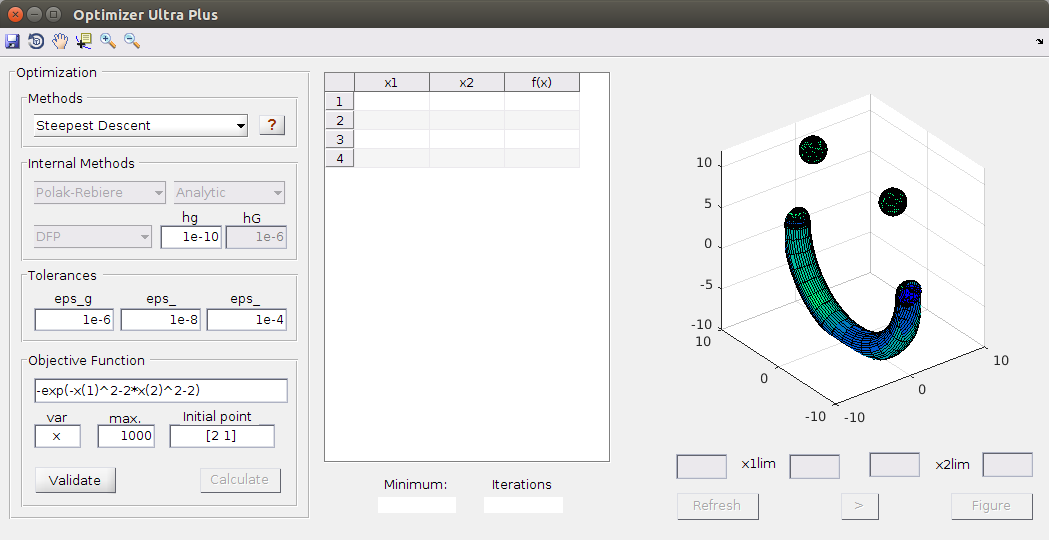
\includegraphics[scale=0.4]{interface.png}
  \caption{Interface Gráfica}
  \label{fig:interface}
\end{figure}

\subsection{Resultados}

Neste relatório, apresenta-se o resultado da convergência em cada um dos cinco métodos para a mesma função, presente na equação \ref{eq:func_obj}. As tolerâncias nos critérios de parada utilizados para gerar os resultados estão descritos na tabela \ref{tab:param}. Em todos os casos, o ponto inicial utilizado foi $x_0=[-2\ 1]$.\\

\begin{equation}
f = (1-x_1)^2 + 2 \,(x_1-x_2^2)^2
\label{eq:func_obj}
\end{equation}
\equationset{Função de Rosenbrock}\\

\begin{table}[!htcb]
  \centering
  \begin{tabular}{|c|c|}
    \hline
    \rowcolor{kugray5}{}
    Tolerância  & Valor\\ \hline
    Relativa ($\epsilon_r$)	&	$1\times10^{-4}$		\\ \hline
    Absoluta ($\epsilon_a$)	&	$1\times10^{-8}$		\\ \hline
    Gradiente ($\epsilon_g$)	&	$1\times10^{-6}$		\\ \hline
  \end{tabular}
  \caption{Tolerâncias para os critérios de parada}
  \label{tab:param}
\end{table}

Outras funções podem ser testadas utilizando a interface gráfica anexa a este relatório, conforme demonstrado na apresentação do trabalho em sala de aula.\\

\section{Método do Gradiente}

%\pagestyle{empty}

\subsection{Descrição}

O método do Gradiente, também chamado de método de descida máxima (MDM), utiliza o conceito de gradiente de uma função vetorial para determinar a direção de avanço. Como o vetor gradiente aponta para a direção de máximo crescimento da função vetorial $f$, o vetor contrário ao gradiente aponta para a direção de máximo decréscimo dessa função.\\

Para encontrar o vetor gradiente de uma função vetorial $f$ deve-se realizar o cálculo analítico ou númerico das derivadas parcias da função para cada variável independente em determeinado. Ou seja,\\

Dado $\emph{f}:  \mathbb{R}^n \rightarrow  \mathbb{R}$ diferenciável no ponto $x^{0} \in \mathbb{R}$:\\

\begin{equation}
\begin{bmatrix}
f_{x_1}^\prime(x^0)\\
f_{x_2}^\prime(x^0)\\
\vdots\\
f_{x_n}^\prime(x^0)
\end{bmatrix} = g(x^0)=\nabla f(x^0) \in \mathbb{R}^n 
\end{equation}\\

A direção de descida para o algoritmo é dada de forma iterativa utilizando o vetor unitário da direção contrária ao gradiente.\\

\begin{equation}
d^k = -\frac{\nabla f(x^k)}{||\nabla f(x^k)||}
\end{equation}\\

Uma vez definida a direção, utiliza-se o método de Brent de busca linear nesta direção para encontrar o passo que realiza a maior descida. Ou seja, o novo ponto $x^{k+1}$ irá depender de $d^k$, $x^k$ e um $\alpha$. Como a direção de descida $d^k$ já foi calculada, e o ponto anterior $x^k$ é conhecido, o novo ponto $x^{k+1}$ depende apenas de $\alpha$.\\

\begin{equation}
\label{busca_linear}
x^{k+1} = x^k+\alpha d^k = x^{k+1}(\alpha)
\end{equation}\\

Dessa forma, podemos escrever o problema da busca linear da seguinte forma:\\

\begin{equation}
\alpha^k = \text{min} \{\tilde{f}(\alpha) = f(x^k+\alpha d^k)\}
\end{equation}\\

Com os três parâmetros conhecidos, é possível calcular novos pontos através de \ref{busca_linear} até o algoritmo atingir um determinado critério de parada.\\

O fluxograma do algoritmo complete pode ser encontrado em \ref{fig:steep}.\\

\emph{Observação: É importante notar que utilizando o método do gradiente, duas direções de descida consecutivas $[d^k\ d^{k+1}]$
são sempre perpendiculares.}\\

\subsection{Resultado}

O método conseguiu encontrar um mínimo em 11 iterações como pode ser visto na tabela \ref{tab:res_stp}. Conforme esperado, as direções de descida estão sempre perpendiculares conforme pode ser observado na figura \ref{fig:res_stp}.

\begin{table}[!htcb]
  \centering
  \begin{tabular}{|c|c|c|c|}
    \hline
    \rowcolor{kugray5}{}
    Iter  & $x(1)$ & $x(2)$ & $f(x)$\\ \hline
 	 0 &  -2.0000	&  1.0000	  &   27.0000\\  \hline
	 1 &  -0.7602	&  -0.6531  &   	5.9148\\  \hline
	 2 &  0.5570	&  0.3348	  &   0.5922\\  \hline
	 3 &  0.4075	&  0.5341	  &   0.3809\\  \hline
	 4 &  1.0287	&  1.0000	  &   0.0025\\  \hline
	 5 &  1.0201	&  1.0114	  &   0.0004\\  \hline
	 6 &  1.0050	&  1.0000	  &   0.0001\\  \hline
	 7 &  1.0035	&  1.0020	  &   0.0000\\  \hline
	 8 &  1.0009	&  1.0000	  &   0.0000\\  \hline
	 9 &  1.0006	&  1.0003	  &   0.0000\\  \hline
	 10 &  1.0001	&  1.0000	  &   0.0000\\  \hline
    \rowcolor{red!40}{}
	 11 &  1.0001	&  1.0001	  &   0.0000\\  \hline
  \end{tabular}
  \caption{Tabela de Resultados: Método do Gradiente}
  \label{tab:res_stp}
\end{table}

\begin{figure}[!htcb]
\centering
\subfigure[Gráfico 3D]{%
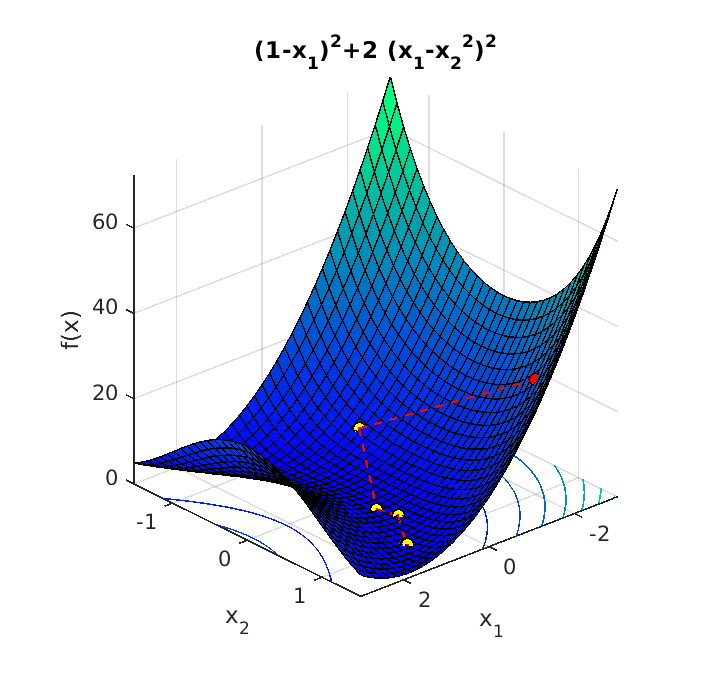
\includegraphics[scale=0.6]{stp_3d_rosen}
\label{fig:subfigure1}}
\quad
\subfigure[Curvas de Nível]{%
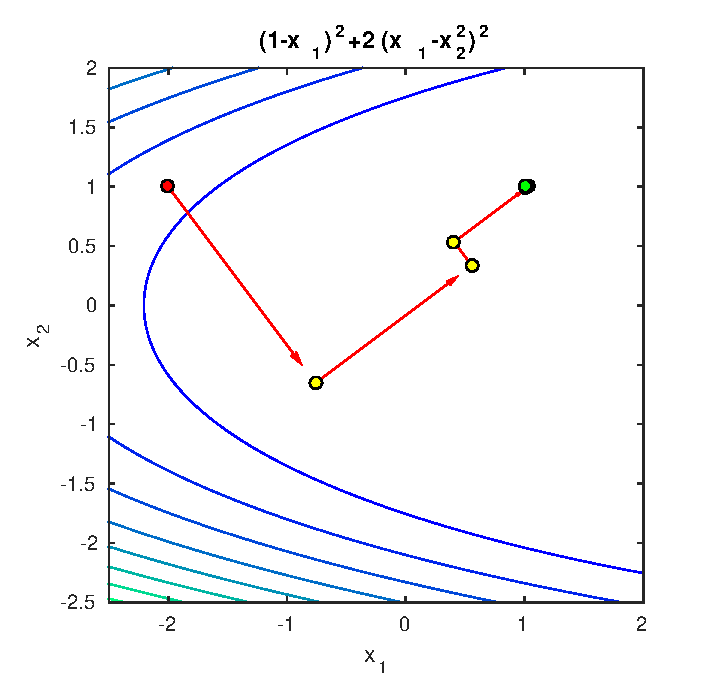
\includegraphics[scale=0.6]{stp_level_rosen}
\label{fig:subfigure2}}
\caption{Método do Gradiente}
\label{fig:res_stp}
\end{figure}

\section{Método do Gradiente Conjugado}

\subsection{Descrição}

O método do gradiente conjugado (MGC) é muito semelhante ao método do gradiente porém tem o objetivo de corrigir problemas de convergência lenta do MDM para problemas mal condicionados. No novo algoritmo, a nova direção de descida é calculada através de uma ponderação entre a direção contrária ao gradiente e a direção de descida calculada na iteração anterior.\\

\begin{equation}
d^{k+1}=-\nabla f(x)+\beta_k d^k
\end{equation}\\

Essa mudança impede que a direção de descida se mova sempre ortogonal, tornando a evolução do algoritmo mais suave.\\

O cálculo de $\beta$ pode ser feito utilizando dois métodos: \emph{Polak-Rebière} ou \emph{Fletcher-Reeves} conforme as equações \eqref{eq:pr} e \eqref{eq:fr}.\\

\begin{equation}
\beta^k = \frac{(g^{k+1})^T(g^{k+1}-g^k)}{g^{k^T}g^k} = \frac{||g^{k+1}||-[g^{k+1}]^Tg^k}{||g^k||}
\label{eq:pr}
\end{equation}
\equationset{\emph{Polak-Rebière}}\\

\begin{equation}
\beta^k = \frac{(g^{k+1})^Tg^k}{g^{k^T}g^k} = \frac{||g^{k+1}||}{||g^k||}
\label{eq:fr}
\end{equation}
\equationset{\emph{Fletcher-Reeves}}\\

O restante do algoritmo segue os mesmos passos do MDM conforme mostrado no fluxograma \ref{fig:grad_conj}.

\subsection{Resultado}

Durante a execução foi utilizado o método de \emph{Polak-Rebière}. O Gradiente Conjudago conseguiu encontrar um mínimo em 7 iterações como pode ser visto na tabela \ref{tab:res_cgrad}. Observa-se que o método encontrou um mínimo diferente do MDM pois possui uma etapa que suaviza a direção de descida impedindo possibilitando direções não perpendiculares como pode ser observado na figura \ref{fig:res_cgrad}.

\begin{table}[!htcb]
  \centering
  \begin{tabular}{|c|c|c|c|}
    \hline
    \rowcolor{kugray5}{}
    Iter  & $x(1)$ & $x(2)$ & $f(x)$\\ \hline
	0     & -2.0000	&  1.0000	&    27.0000\\ \hline
	1     & -0.7602	&  -0.6531  &  	5.9148\\ \hline
	2     & 0.3566	&  -0.2932  &  	0.5604\\ \hline
	3     & 0.7883	&  -0.9225  &  	0.0527\\ \hline
	4     & 1.0059	&  -1.0115  &  	0.0006\\ \hline
	5     & 1.0094	&  -1.0052  &  	0.0001\\ \hline
	6     & 1.0015	&  -0.9998  &  	0.0000\\ \hline
	\rowcolor{red!40}{}	
	7     & 0.9999	&  -0.9999  &  	0.0000\\ \hline
  \end{tabular}
  \caption{Tabela de Resultados: Método do Gradiente Conjugado}
  \label{tab:res_cgrad}
\end{table}

\begin{figure}[!htcb]
\centering
\subfigure[Gráfico 3D]{%
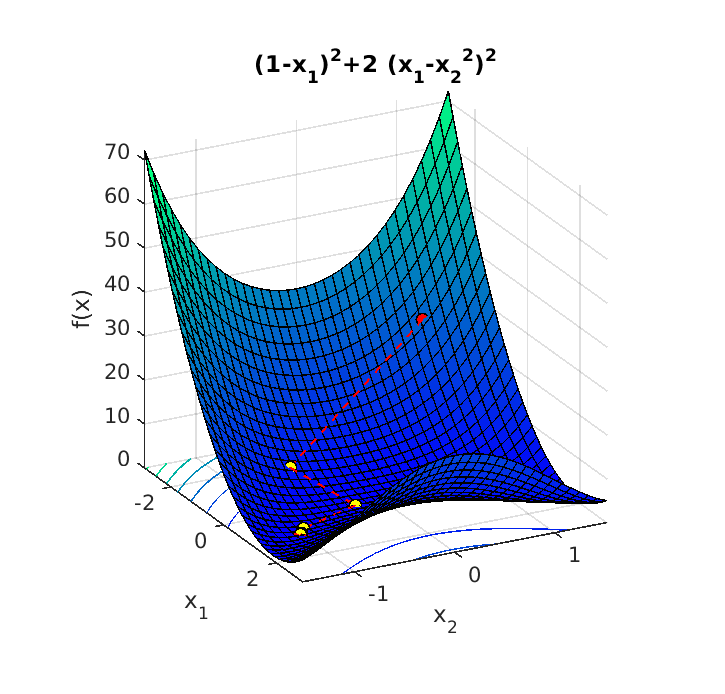
\includegraphics[scale=0.6]{cgrad_3d_rosen}
\label{fig:subfigure1}}
\quad
\subfigure[Curvas de Nível]{%
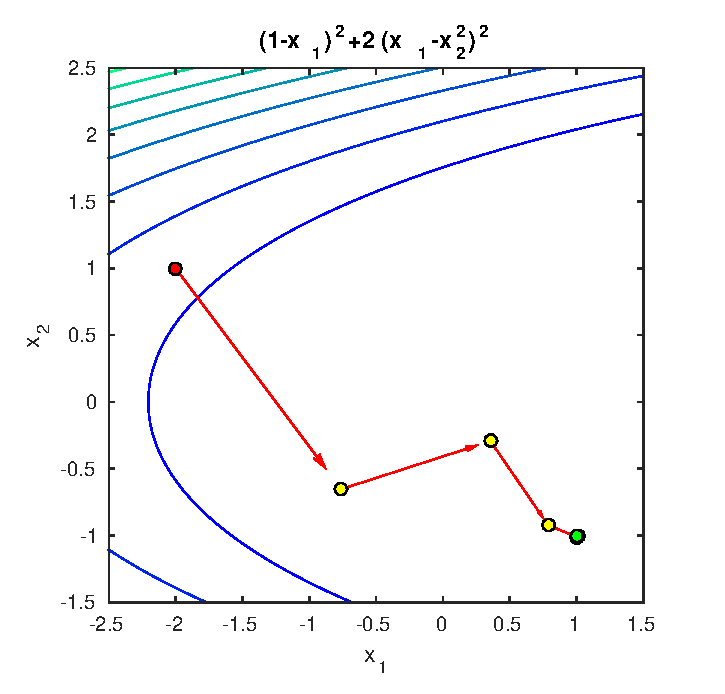
\includegraphics[scale=0.6]{cgrad_level_rosen}
\label{fig:subfigure2}}
\caption{Método do Gradiente Conjugado}
\label{fig:res_cgrad}
\end{figure}

\section{Método de Newton}

\subsection{Descrição}

Os métodos de Newton são baseados na minimização de funções quadráticas, sendo a função $f(x)$ aproximada por uma quadrática a cada iteração. Como o mínimo de funções quadráticas é bem conhecido, segue que este mínimo é utilizado como passo para a nova iteração.\\

Para executar o método de Newton é necessário conhecimento do vetor gradiente $g(x)$ e da matriz Hessiana $G(x)$. Ambos podem ser obtidos analiticamente ou numéricamente.\\

Para encontrar a matriz Hessiana de uma função vetorial $f$ deve-se realizar o cálculo analítico ou númerico das derivadas parcias do gradiente para cada variável independente em determinado ponto. Ou seja,\\

Dado $\emph{f}:  \mathbb{R}^n \rightarrow  \mathbb{R} \in \mathbb{C}^2$ e $x^{0} \in \mathbb{R}^n$:

\begin{equation}
\begin{bmatrix}
f_{x_1x_1}^\prime\prime(x^0) & f_{x_1x_2}^\prime\prime(x^0) & \hdots & f_{x_1x_n}^\prime\prime(x^0)\\
f_{x_2x_1}^\prime\prime(x^0) & f_{x_2x_2}^\prime\prime(x^0) & \hdots & f_{x_2x_n}^\prime\prime(x^0)\\
\vdots & & \ddots &\\
f_{x_nx_1}^\prime\prime(x^0) & f_{x_nx_2}^\prime\prime(x^0) & \hdots & f_{x_nx_n}^\prime\prime(x^0)\\
\end{bmatrix} = \nabla^2f(x^0)=H(x^0) = G(x^0)
\end{equation}\\

Utilizando os conhecimentos prévios de funções quadráticas é fácil notar que o mínimo para funções do tipo $f(x)=\frac{1}{2}x^TAx + x^Tb$ com $A>0$ é $x^*=-A^{-1}b$. A série de Taylor também fornece uma aproximação de segunda ordem para funções vetoriais conforme a equação \eqref{eq:taylor}.\\

\begin{align}
f_{quad}(x)&= f(x^k)+(x-x^k)^T\nabla f(x^k) + \frac{1}{2}(x-x^k)^T\nabla^2f(x^k)(x-x^k)\\
&=f(x^k)+(x-x^k)^Tg(x^k) + \frac{1}{2}(x-x^k)^TG(x^k)(x-x^k)
\label{eq:taylor}
\end{align}
\equationset{\emph{Aproximação de segunda ordem por Taylor}}\\

A aproximação quadrática de $f(x)$ para $G(x)>0$ possui mínimo em $(x-x^k)^*=-[G^k]^{-1}g^k$. Dessa forma, o ponto para nova é atualizado através de \eqref{eq:newton}.\\

\begin{eqnarray}
x^{k+1} = x^k + d^k\\
d^k = -[G^k]^{-1}g^k
\label{eq:newton}
\end{eqnarray}\\

Uma vez definida a regra para atualização de $x^k$ basta executar o algoritmo de forma iterativa conforme o fluxograma \ref{fig:newton_flux}.

\subsection{Resultado}

Durante a execução do algoritmo foi utilizado o cálculo analítico (simbólico) do Gradiente e da Hessiana da função vetorial. O método encontrou o mínimo em apenas uma iteração como pode ser visto na tabela \ref{tab:res_newton}. Isso acontece pois a direção de descida é dado por uma aproximação de segunda ordem da função que nesse caso se encaixa corretamente com a função. Esse resultado pode ser observado graficamente na figura \ref{fig:res_newton}.

\begin{table}[!htcb]
  \centering
  \begin{tabular}{|c|c|c|c|}
    \hline
    \rowcolor{kugray5}{}
    Iter  & $x(1)$ & $x(2)$ & $f(x)$\\ \hline
	0 & -2.0000  & 	1.0000	& 27.0000\\ \hline
	\rowcolor{red!40}{}	
	1 &  1.0000	 & 1.0000	& 0.0000\\ \hline
  \end{tabular}
  \caption{Tabela de Resultados: Método de Newton}
  \label{tab:res_newton}
\end{table}

\begin{figure}[!htcb]
\centering
\subfigure[Gráfico 3D]{%
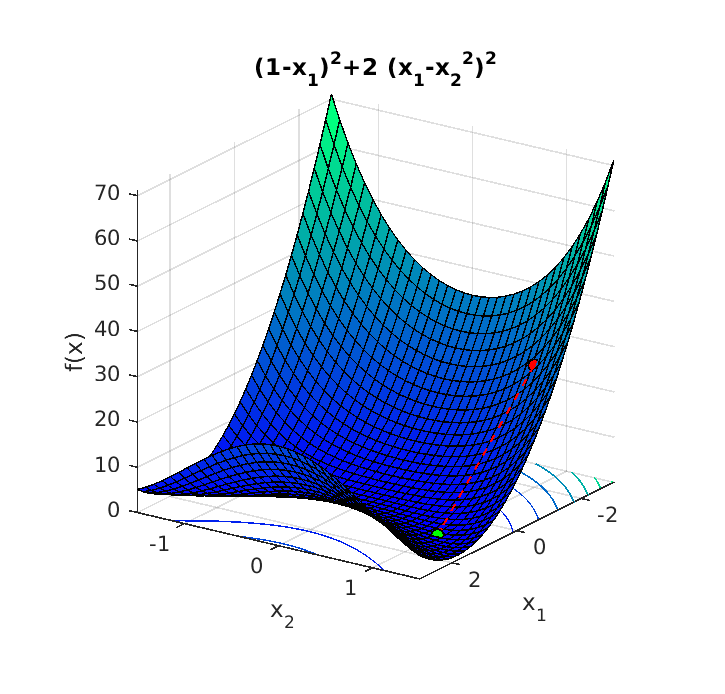
\includegraphics[scale=0.6]{newton_3d_rosen}
\label{fig:subfigure1}}
\quad
\subfigure[Curvas de Nível]{%
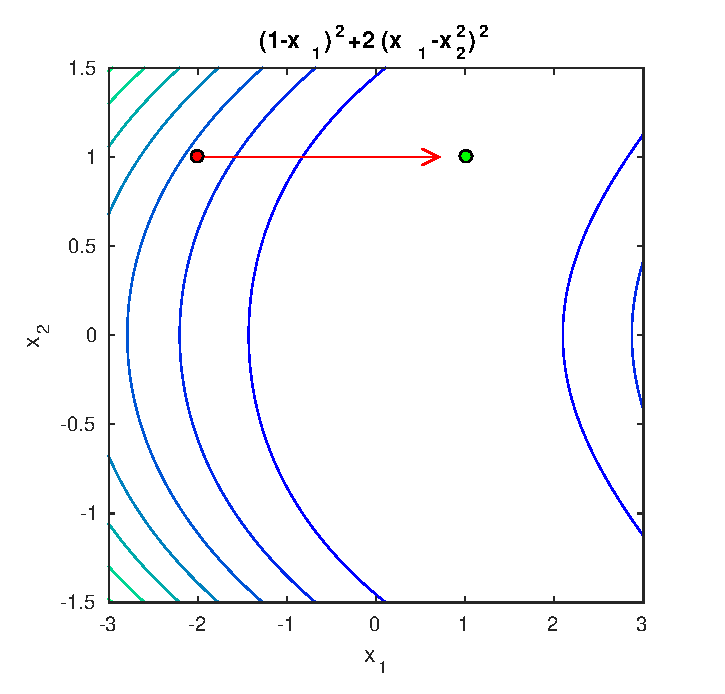
\includegraphics[scale=0.6]{newton_level_rosen}
\label{fig:subfigure2}}
\caption{Método de Newton}
\label{fig:res_newton}
\end{figure}

\section{Método de Newton Modificado}
\subsection{Descrição}

O método de Newton modificado foi criado para contornar problemas de convergência quando a Hessiana da função objetivo não é definida positiva. O algoritmo verifica se a Hessiana é positiva definida ou não em determinado ponto. Se ela for definida positiva, o algoritmo segue de forma equivalente ao método de Newton. Caso contrário, é feita uma correção nos autovalores da Hessiana somando uma matriz identida vezes um $\gamma$ conforme a equação \eqref{eq:newton_mod}.\\

\begin{equation}
F^k = G^k + \gamma \mathbb{I}_n
\label{eq:newton_mod}
\end{equation}
\equationset{Correção da Hesssiana}\\

Se a Hessiana for positiva definida $\gamma=0$, porém se ela não for positiva definida, $\gamma$ deverá ser grande o suficiente tal que todos os autovalores de $F$ sejam maiores que $0$, tornando a Hessiana positiva definida. Ou seja:\\

\begin{equation}
\gamma \in \mathbb{R} | \lambda_i(G^k+\gamma \mathbb{I}_n)>0
\end{equation}\\

Com isso, a direção de descida passa a ser $d^k=-[F]^{-1}g(k)$\\

O restante do algoritmo funciona da mesma forma conforme pode ser observado no fluxograma \ref{fig:newton_mod_flux}.\\


\subsection{Resultado}

Da mesma forma que o Método de Newton, o Método de Newton Modificado também encontra o mínimo com apenas uma iteração como pode ser visto na tabela \ref{tab:res_newtonmod}. Esse resultado era esperado pois a modificação feita no método tem o objetivo de contornar problemas de convergência apenas. Em situações onde o Método de Newton converge, o modificado irá convergir da mesma forma.\\

\begin{table}[!htcb]
  \centering
  \begin{tabular}{|c|c|c|c|}
    \hline
    \rowcolor{kugray5}{}
    Iter  & $x(1)$ & $x(2)$ & $f(x)$\\ \hline
	0 & -2.0000  & 	1.0000	& 27.0000\\ \hline
	\rowcolor{red!40}{}	
	1 &  1.0000	 & 1.0000	& 0.0000\\ \hline
  \end{tabular}
  \caption{Tabela de Resultados: Método de Newton Modificado}
  \label{tab:res_newtonmod}
\end{table}

\begin{figure}[!htcb]
\centering
\subfigure[Gráfico 3D]{%
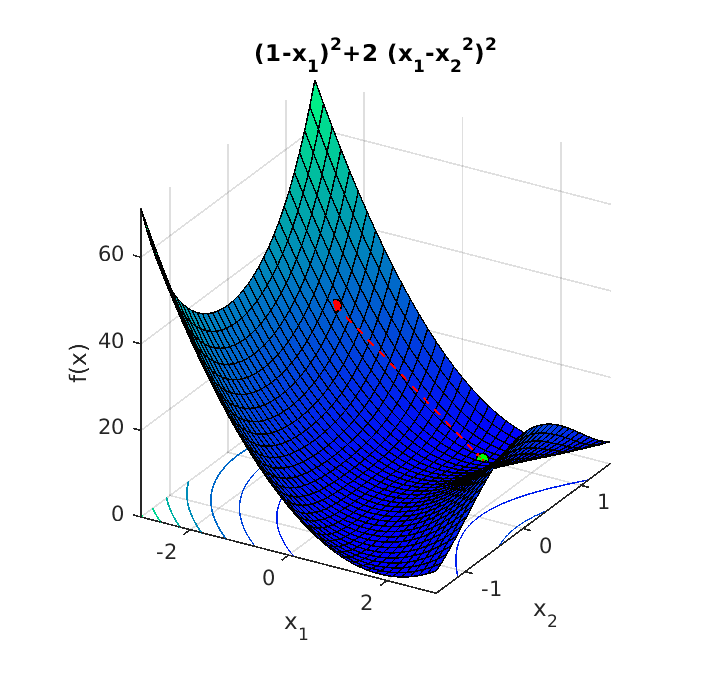
\includegraphics[scale=0.6]{newtonmod_3d_rosen}
\label{fig:subfigure1}}
\quad
\subfigure[Curvas de Nível]{%
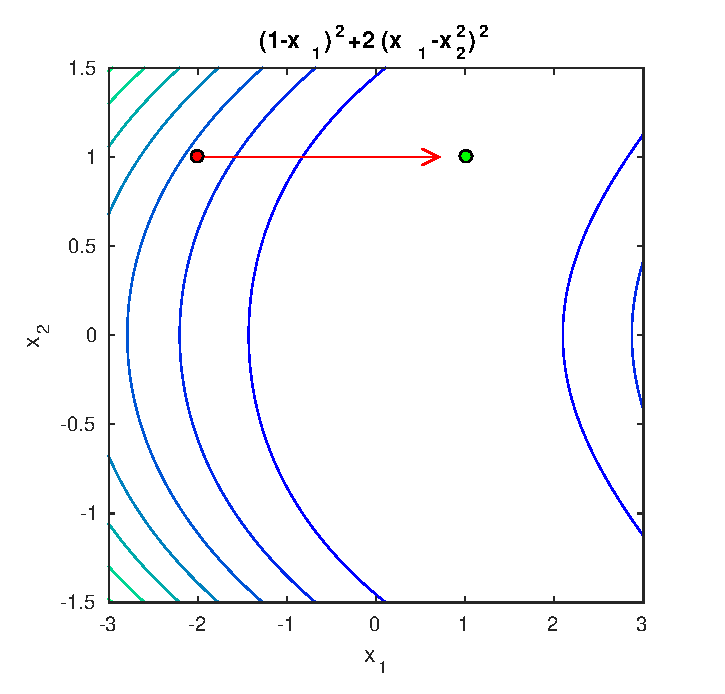
\includegraphics[scale=0.6]{newtonmod_level_rosen}
\label{fig:subfigure2}}
\caption{Método de Newton Modificado}
\label{fig:res_newtonmod}
\end{figure}


\section{Método de Quasi-Newton}
\subsection{Descrição}

O objetivo do método de Quasi-Newton é facilitar o cálculo da inversa da Hessiana, uma vez que derivar duas vezes a função $f$ e ainda fazer a inversão da matriz Hessiana são tarefas extremamente custosas.\\

\begin{equation}
H = [G^k]^{-1}
\end{equation}\\

Portanto, nesse método, são utilizadas aproximação para a inversa da Hessiana. Nesse contexto, duas aproximações são propostas: A de \emph{Davidon-Fletcher-Powell} (DFP) e a de \emph{Broyden-Fletcher-Goldfarb-Shanno} (BFGS).\\

\begin{equation}
H^{k+1} = H^k - \frac{H\gamma\gamma^TH}{\gamma^T\gamma}+ \frac{\delta\delta^T}{\delta^T\gamma}
\end{equation}
\equationset{\emph{Davidon-Fletcher-Powell}}\\

\begin{equation}
H^{k+1} = H^k - \frac{\delta \gamma^T H + H \gamma \delta^T}{\delta^T\gamma}+ \left( 1 + \frac{\gamma^T H \gamma}{\delta^T\gamma} \right)\frac{\delta\delta^T}{\delta^T\gamma}
\end{equation}
\equationset{\emph{Broyden-Fletcher-Goldfarb-Shanno}}\\

Onde $\delta^k=x^{k+1}-x^k$ e $\gamma^k=g^{k+1}-g^k$\\

O restante do algoritmo funciona de forma equivalente ao método de Newton conforme explicitado no fluxograma \ref{fig:quasi_newton_flux}.\\


\subsection{Resultado}

Durante a execução do algoritmo foi utilizado método de DFP para o cálculo aproximado da Hessiana. O método encontrou o mínimo em 6 iteraçõse como pode ser visto na tabela \ref{tab:res_quasinewton}. Isso acontece devido ao cálculo aproximado da Hessiana que dificulta a entrada no critério de parada como pode ser visto na figura \ref{fig:res_quasinewton}.\\

\begin{table}[!htcb]
  \centering
  \begin{tabular}{|c|c|c|c|}
    \hline
    \rowcolor{kugray5}{}
    Iter  & $x(1)$ & $x(2)$ & $f(x)$\\ \hline
	 0  & -2.0000   &   	1.0000	  &  27.0000\\ \hline
	 1 	& -0.7602   &   	-0.6531  &  	5.9148\\ \hline
	 2  & 0.3566	   &   -0.2932  &  	0.5604\\ \hline
	 3  & 0.9398	   &   -0.9812  &  	0.0047\\ \hline
	 4  & 0.9757	   &   -0.9815  &  	0.0009\\ \hline
	 5  & 0.9998	   &   -1.0000  &  	0.0000\\ \hline
	 6  & 1.0000	   &   -1.0000  &  	0.0000\\ \hline
	\rowcolor{red!40}{}	
	 7  & 1.0000	   &   -1.0000  &  	0.0000\\ \hline
  \end{tabular}
  \caption{Tabela de Resultados: Método de Quasi-Newton}
  \label{tab:res_quasinewton}
\end{table}

\begin{figure}[!htcb]
\centering
\subfigure[Gráfico 3D]{%
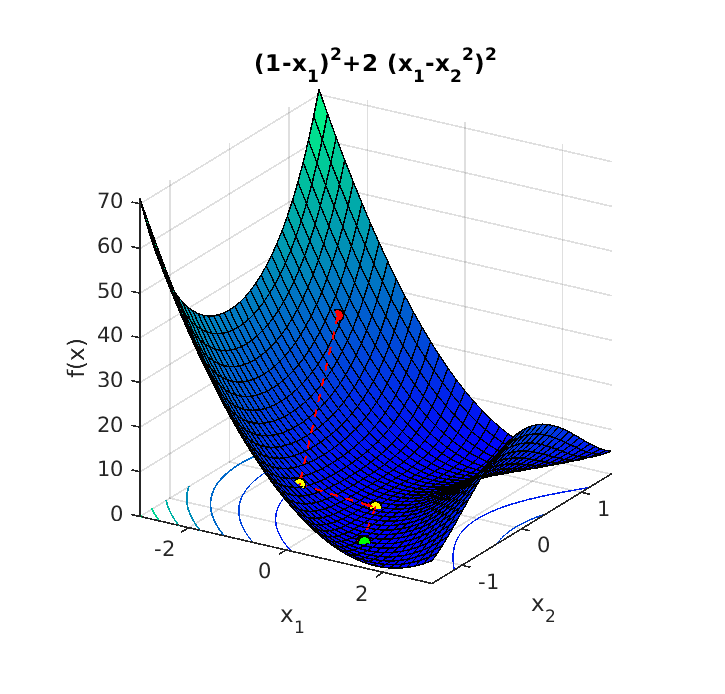
\includegraphics[scale=0.6]{quasinewton_3d_rosen}
\label{fig:subfigure1}}
%\quad
\subfigure[Curvas de Nível]{%
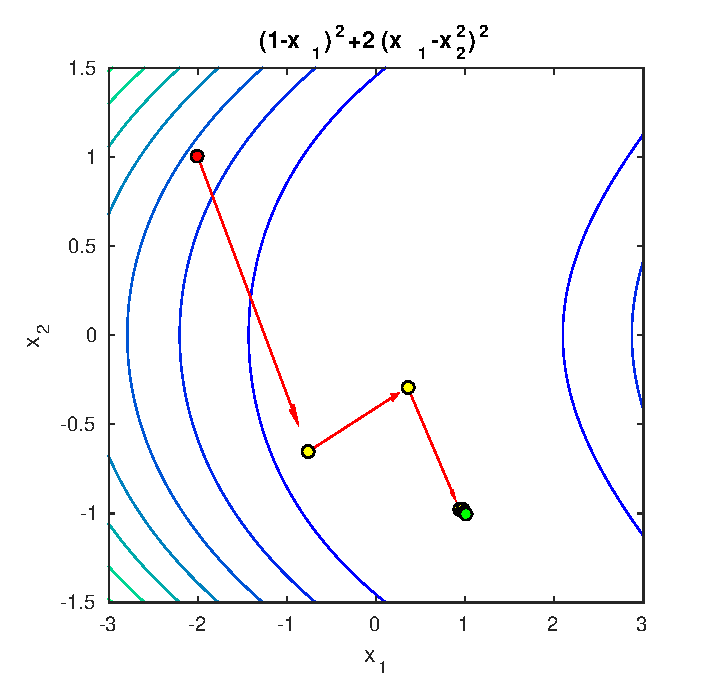
\includegraphics[scale=0.6]{quasinewton_level_rosen}
\label{fig:subfigure2}}
\caption{Método de Quasi-Newton}
\label{fig:res_quasinewton}
\end{figure}

\section{Resultados Complementares}

\subsection{Outras funções de duas variáveis}

Além dos resultados apresentados para comparação entre os métodos, foram feitos também testes em outras funções. Esses testes apresentam resultados gráficos interessantes permitinido melhor visualização do funcionamento dos métodos.\\

Um dos exemplos executados durante a apresentação do trabalho foi a utilização da Gradiente Conjugado para a função \eqref{eq:func_comp}.\\

\begin{equation}
f = -e^{(-x_1^2-2x_2^2-2)}
\label{eq:func_comp}
\end{equation}
\equationset{Função Exponencial}\\

O resultado mostrado na figura \ref{fig:res_cgrad_exp} descreve claramente como o gradiente conjugado suaviaza a direção de descida do gradiente seguindo uma trajetória curva.\\

\begin{figure}[!htcb]
\centering
\subfigure[Gráfico 3D]{%
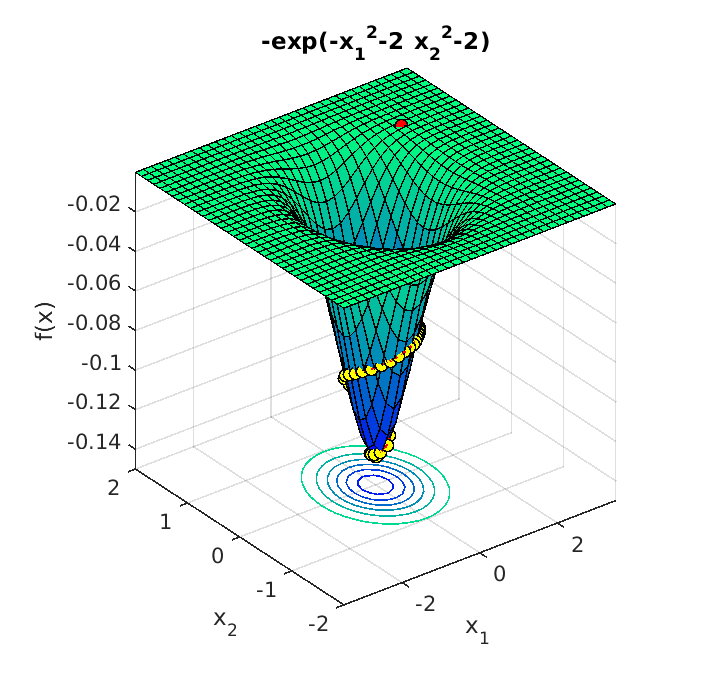
\includegraphics[scale=0.6]{cgrad_3d_exp}
\label{fig:subfigure1}}
\quad
\subfigure[Curvas de Nível]{%
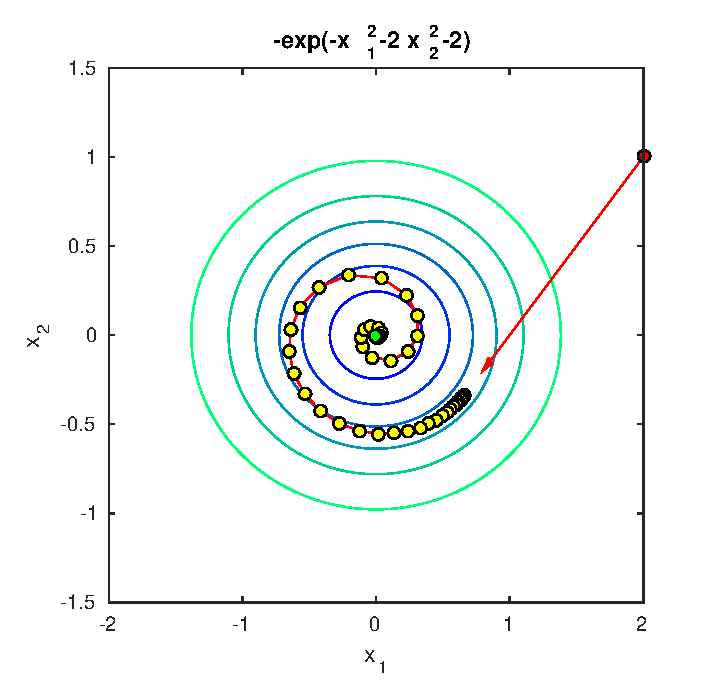
\includegraphics[scale=0.6]{cgrad_level_exp}
\label{fig:subfigure2}}
\caption{Gradiente Conjugado aplicado a função exponencial}
\label{fig:res_cgrad_exp}
\end{figure}

Outro resultado interessante obtido com o Gradiente Conjugado aparece ao aplicar o método à função \eqref{eq:func_sin}.\\

\begin{equation}
f = {sin(x_1)}^2+{sin(x_2)}^2
\label{eq:func_sin}
\end{equation}
\equationset{Função Seno}\\

O resultado apresentado na figura \ref{fig:res_cgrad_sin} mostra que a função possui infinitos mínimos locais. O algoritmo naturalmente encontra o mínimo mais próximo do ponto inicial.\\

\begin{figure}[!htcb]
\centering
\subfigure[Gráfico 3D]{%
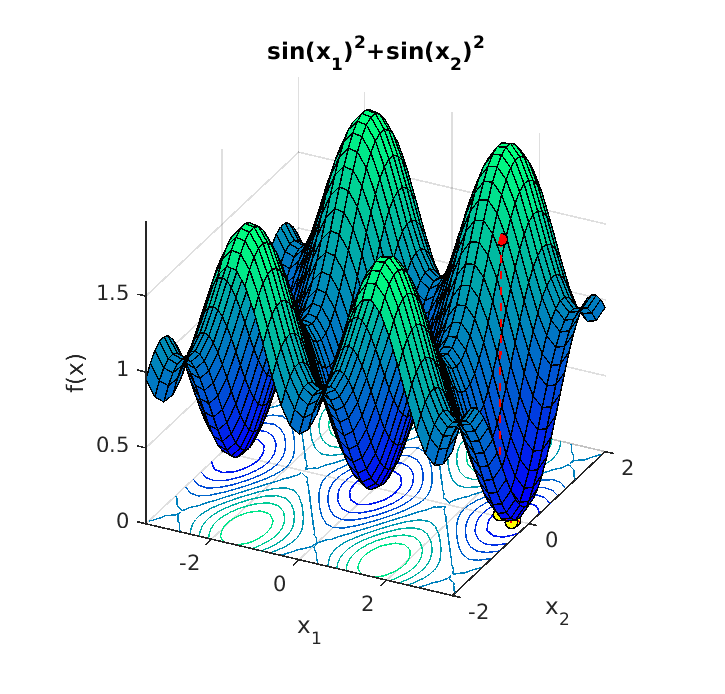
\includegraphics[scale=0.6]{cgrad_3d_sin}
\label{fig:subfigure1}}
\quad
\subfigure[Curvas de Nível]{%
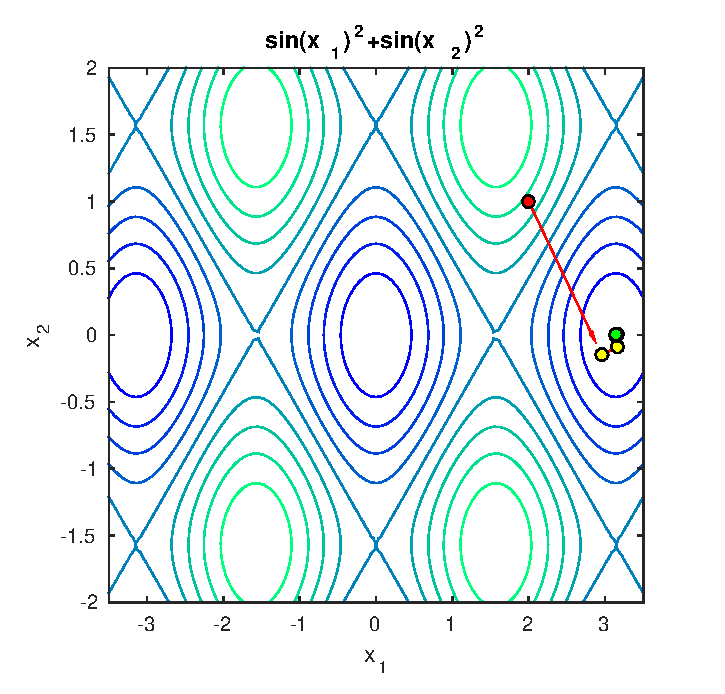
\includegraphics[scale=0.6]{cgrad_level_sin}
\label{fig:subfigure2}}
\caption{Gradiente Conjugado aplicado a função seno}
\label{fig:res_cgrad_sin}
\end{figure}

Outro resultado interessante para a função seno é que, por não ser uma função positiva definida, a Hessiana por vezes não necessáriamente garante a convergência para um mínimo. Pelo método de Newton, que utiliza a Hessiana pura, podemos convergir para um ponto de máximo ou de sela. No entanto, usando o método de Newton-Modificado ou o Quase-Newton, conseguimos contornar esse problema garantindo uma "Hessiana" sempre positiva definida.

\subsection{Funções com mais de duas variáveis}

Durante todo o relatório foram apresentados apenas resultados para funções bivariáveis. O motivo é que para essas funções a exibição dos resultados é muito mais agradável.\\

Entretanto, a interface criada permite também a utilização de funções como mais de duas variáveis, apresentando novamente a tabela com os resultados da otimização. Já os gráficos não podem ser gerados como anteriormente portanto foi utilizada a abordagem de mostrar o decaimento da função objetivo e do módulo do gradiente no tempo (iterações).\\

O módulo do gradiente indo para zero indica que um ponto de extremo foi atingido. Dessa forma, avaliando os dois gráficos é possível identificar se a função foi para algum ponto de mínimo.\\

A função utilizada para teste foi a função exponencial \eqref{eq:func_3var} com três variáveis. Foi utilizado o Método do Gradiente com ponto inicial $x_0=[2\ 1\ 1]$.\\

\begin{equation}
f = -e^{(-x_1^2-2x_2^2- x_3^2 -2)}
\label{eq:func_3var}
\end{equation}
\equationset{Função Exponencial}\\

O método encontrou o mínimo em 4 iteração como pode ser visto na tabela \ref{tab:res_3vars}. O resultado gráfico para o algoritmo, conforme descrito anteriormente, mostra o valor da função objetivo e o módulo do gradiente. Analisando a figura \ref{fig:res_3vars} é possível ver claramente a função decaindo com o número de iterações até o módulo do gradiente chegar a zero.\\

\begin{table}[!htcb]
  \centering
  \begin{tabular}{|c|c|c|c|c|}
    \hline
    \rowcolor{kugray5}{}
    Iter  & $x(1)$ & $x(2)$ & $x(3)$ & $f(x)$\\ \hline
	0   &  2.0000  & 	1.0000  &	1.0000	&  -0.0001\\ \hline
	1   & 0.6154	  & -0.3846  &	0.3077	&  -0.0627\\ \hline  
	2   & 0.2198  & 	0.1099  &	0.1099	&  -0.1244\\ \hline
	3   & 0.0676	  & -0.0423  &	0.0338	&  -0.1341\\ \hline  
	4   & 0.0242  & 	0.0121  &	0.0121	&  -0.1352\\ \hline
	\rowcolor{red!40}{}	
	5   & 0.0074	  & -0.0046  &	0.0037	&  -0.1353\\ \hline
  \end{tabular}
  \caption{Tabela de Resultados: Método do Gradiente para três variáveis}
  \label{tab:res_3vars}
\end{table}

\begin{figure}[!htcb]
\centering
\subfigure[Evolução da função objetivo]{%
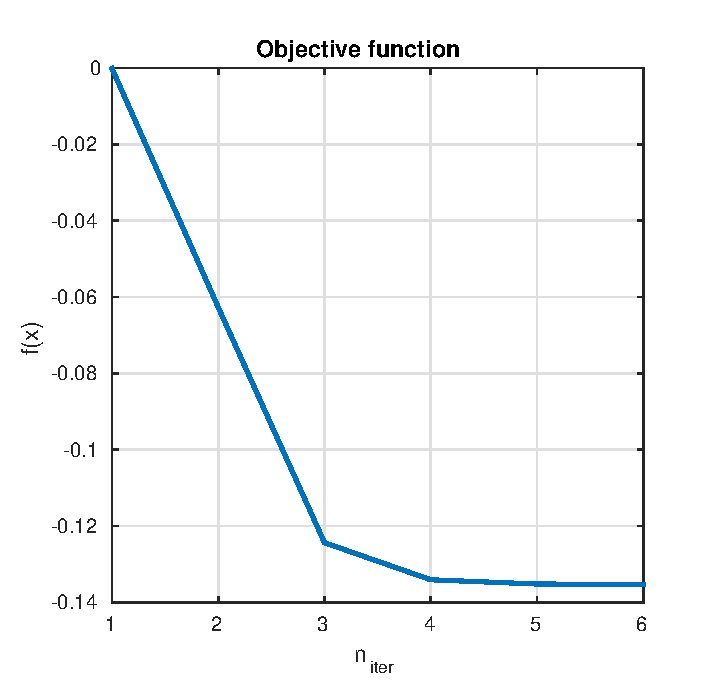
\includegraphics[scale=0.6]{3vars_objfun}
\label{fig:subfigure1}}
\quad
\subfigure[Evolução da norma do Gradiente]{%
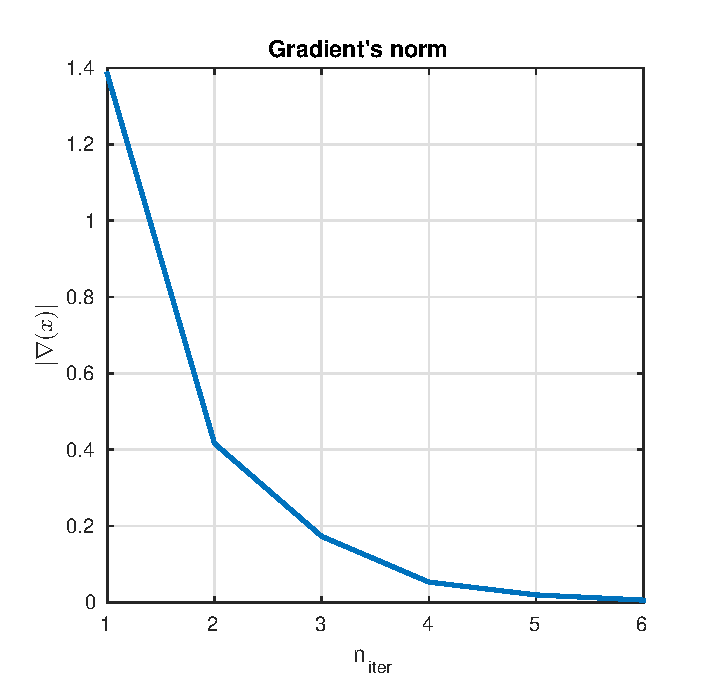
\includegraphics[scale=0.6]{3vars_grad}
\label{fig:subfigure2}}
\caption{Método do Gradiente para três variáveis}
\label{fig:res_3vars}
\end{figure}

\section{Fluxogramas}

%\subsection{Método do Gradiente}
\begin{figure}[!hctb]
\centering
\scalebox{0.85}{% Define block styles
\tikzstyle{io} = [trapezium,trapezium left angle=70,trapezium right angle=-70,minimum height=1.5cm, draw, fill=yellow!20, text width=11em, text badly centered, node distance=2cm, inner sep=0pt]
\tikzstyle{decision} = [diamond, draw, fill=red!20, 
    text width=6em, text badly centered, node distance=3.5cm, inner sep=0pt]
\tikzstyle{decision2} = [diamond, draw, fill=red!20, 
    text width=9em, text badly centered, node distance=4.5cm, inner sep=0pt]
\tikzstyle{block} = [rectangle, draw, fill=blue!20, node distance=4cm,
    text width=10em, text centered, rounded corners, minimum height=4em]
    \tikzstyle{block0} = [rectangle, draw, fill=blue!20, 
    text width=4em, text centered, rounded corners, minimum height=2em]
    \tikzstyle{block1} = [rectangle, draw, fill=blue!20, node distance=2cm,
    text width=7em, text centered, rounded corners, minimum height=4em]
    \tikzstyle{line} = [draw, -latex']
\tikzstyle{cloud} = [draw, ellipse,fill=green!20, node distance=2cm,
    minimum height=2em]
    \tikzstyle{io2} = [trapezium,trapezium left angle=70,trapezium right angle=-70,minimum height=0.7cm, draw, fill=yellow!20, text width=1.6cm, text badly centered, node distance=3.5cm, inner sep=0pt]
    
\begin{tikzpicture}[node distance = 2cm, auto]
    % Place nodes
    \node [io] (input) {$x^0 \in \mathbb{R}^n$: ponto partida\\$\varepsilon_g,\varepsilon_a,\varepsilon_r$: toler\^ancias};
    \node [block0, below of =input] (init) {$x^k = x^0$};
    \node [block1, below of =init] (grad) {$\nabla f(x_k)=g(x_k)$};
    \node [decision, below of=grad] (evaluate) {$|g(x_k)|< \varepsilon_g $};
    \node [block, below of=evaluate] (direct) {$d^k=-\frac{g(x_k)}{||g(x_k)||}$\\$\tilde{f}(\alpha)=f(x^k+\alpha \, d^k)$\\$\alpha_k = min\{\tilde{f}(\alpha)\}$\\$x^{k+1}=x^k+\alpha_k \, d^k$};
    \node [decision2, below of=direct] (evaluate2) {$|f(x^{k+1})-f(x^k)|<\varepsilon_a +\varepsilon_r \, |f(x^k)|$};
    \node [block1,left of = evaluate, node distance = 4cm] (reinit) {$x^k = x^{k+1}$};    
    \node [io2, below of=evaluate2] (out) {$x_{min}=x$};
    \node [cloud,below of = out] (stop) {FIM};
         
    % Draw edges
    \path [line] (input) -- (init);
    \path [line] (init) -- (grad);
    \path [line] (grad) -- (evaluate);
    \path [line,rounded corners] (evaluate.east)-- ++(20mm,0mm) |- node [near start] {sim} (out.east);
    \path [line] (evaluate) -- node [near start] {não}(direct);
    \path [line] (direct) -- (evaluate2);
    \path [line] (evaluate2) -- node [near start] {sim} (out);
    \path [line,rounded corners] (evaluate2.west) -| node [near start] {não} (reinit);
    \path [line,rounded corners] (reinit) |- (grad.west);
    \path [line] (out) -- (stop);
\end{tikzpicture}}
\caption{Método de Descida Máxima (Gradiente)}
\label{fig:steep}
\end{figure}

%\subsection{Método do Gradiente Conjugado}

\begin{figure}[!hctb]
\centering
\scalebox{0.85}{% Define block styles
\tikzstyle{io} = [trapezium,trapezium left angle=70,trapezium right angle=-70,minimum height=1.5cm, draw, fill=yellow!20, text width=11em, text badly centered, node distance=2cm, inner sep=0pt]
\tikzstyle{decision} = [diamond, draw, fill=red!20, 
    text width=6em, text badly centered, node distance=3.5cm, inner sep=0pt]
\tikzstyle{decision2} = [diamond, draw, fill=red!20, 
    text width=9em, text badly centered, node distance=4.5cm, inner sep=0pt]
\tikzstyle{block} = [rectangle, draw, fill=blue!20, node distance=3.5cm,
    text width=10em, text centered, rounded corners, minimum height=4em]
    \tikzstyle{block0} = [rectangle, draw, fill=blue!20, 
    text width=4em, text centered, rounded corners, minimum height=2em]
    \tikzstyle{block1} = [rectangle, draw, fill=blue!20, node distance=2cm,
    text width=7em, text centered, rounded corners, minimum height=4em]
    \tikzstyle{block2} = [rectangle, draw, fill=blue!20, node distance=4cm,
    text width=12em, text centered, rounded corners, minimum height=4em]
    \tikzstyle{line} = [draw, -latex']
\tikzstyle{cloud} = [draw, ellipse,fill=green!20, node distance=2cm,
    minimum height=2em]
    \tikzstyle{io2} = [trapezium,trapezium left angle=70,trapezium right angle=-70,minimum height=0.7cm, draw, fill=yellow!20, text width=1.6cm, text badly centered, node distance=3.5cm, inner sep=0pt]
    
\begin{tikzpicture}[node distance = 2cm, auto]
    % Place nodes
    \node [io] (input) {$x^0 \in \mathbb{R}^n$: ponto partida\\$\varepsilon_g,\varepsilon_a,\varepsilon_r$: toler\^ancias};
    \node [block0, below of =input] (init) {$x^k = x^0$};
    \node [block1, below of =init] (grad) {$\nabla f(x_k)=g(x_k)$};
    \node [decision, below of=grad] (evaluate) {$|g(x_k)|< \varepsilon_g $};
    \node [block2, below of=evaluate] (direct_conj) {$d^k=-\frac{g(x_k)}{||g(x_k)||}$ \\ $\beta$: $\begin{cases}$ Polak - Rebière $\,  ou\\ $Fletcher -Reeves$\end{cases}$\\$d^k=d^k+\beta \, d^{k-1}$};
    \node [block, below of=direct_conj] (direct) {$\tilde{f}(\alpha)=f(x^k+\alpha \, d^k)$\\$\alpha_k = min\{\tilde{f}(\alpha)\}$\\$x^{k+1}=x^k+\alpha_k \, d^k$}; 
    \node [decision2, below of=direct] (evaluate2) {$|f(x^{k+1})-f(x^k)|<\varepsilon_a +\varepsilon_r \, |f(x^k)|$};
    \node [block1,left of = evaluate, node distance = 4cm] (reinit) {$x^k = x^{k+1}$};    
    \node [io2, below of=evaluate2] (out) {$x_{min}=x$};
    \node [cloud,below of = out] (stop) {FIM};
   
       
    % Draw edges
    \path [line] (input) -- (init);
    \path [line] (init) -- (grad);
    \path [line] (grad) -- (evaluate);
    \path [line,rounded corners] (evaluate.east)-- ++(20mm,0mm) |- node [near start] {sim} (out.east);
     \path [line] (evaluate) -- node [near start] {nao}(direct_conj);
    \path [line] (direct_conj) -- (direct);
    \path [line] (direct) -- (evaluate2);
    \path [line] (evaluate2) -- node [near start] {sim} (out);
    \path [line,rounded corners] (evaluate2.west) -| node [near start] {não} (reinit);
    \path [line,rounded corners] (reinit) |- (grad.west);
    \path [line] (out) -- (stop);
\end{tikzpicture}}
\caption{Método do Gradiente Conjugado}
\label{fig:grad_conj}
\end{figure}

%\subsection{Método de Newton}

\begin{figure}[!hct]
\centering
\scalebox{0.85}{% Define block styles
\tikzstyle{io} = [trapezium,trapezium left angle=70,trapezium right angle=-70,minimum height=1.5cm, draw, fill=yellow!20, text width=11em, text badly centered, node distance=2cm, inner sep=0pt]
\tikzstyle{decision} = [diamond, draw, fill=red!20, 
    text width=6em, text badly centered, node distance=3cm, inner sep=0pt]
\tikzstyle{decision2} = [diamond, draw, fill=red!20, 
    text width=9em, text badly centered, node distance=4cm, inner sep=0pt]
\tikzstyle{block} = [rectangle, draw, fill=blue!20, node distance=3cm,
    text width=10em, text centered, rounded corners, minimum height=4em]
\tikzstyle{block2} = [rectangle, draw, fill=blue!20, node distance=3cm,
    text width=15em, text centered, rounded corners, minimum height=4em]
    \tikzstyle{block0} = [rectangle, draw, fill=blue!20, 
    text width=4em, text centered, rounded corners, minimum height=2em]
    \tikzstyle{block1} = [rectangle, draw, fill=blue!20, node distance=2cm,
    text width=8em, text centered, rounded corners, minimum height=4em]
    \tikzstyle{line} = [draw, -latex']
\tikzstyle{cloud} = [draw, ellipse,fill=green!20, node distance=2cm,
    minimum height=2em]
    \tikzstyle{io2} = [trapezium,trapezium left angle=70,trapezium right angle=-70,minimum height=0.7cm, draw, fill=yellow!20, text width=1.6cm, text badly centered, node distance=3.5cm, inner sep=0pt]
    
\begin{tikzpicture}[node distance = 2cm, auto]
    % Place nodes
    \node [io] (input) {$x^0$: ponto de partida\\$\varepsilon_g,\varepsilon_a,\varepsilon_r$: tolerâncias};
    \node [block0, below of =input] (init) {$x^k = x^0$};
    \node [block1, below of =init] (grad) {$\nabla f(x_k)=g(x_k)$\\$\nabla^2 f(x_k)=G(x_k)$};
    \node [decision, below of=grad] (evaluate) {$|g(x_k)|< \varepsilon_g $};
    \node [block, below of=evaluate] (direct) {$d^k=-[G^k]^{-1} \, g^k$\\ $x^{k+1}=x^k+d^k$};
    \node [decision2, below of=direct] (evaluate2) {$|f(x^{k+1})-f(x^k)|<\varepsilon_a +\varepsilon_r \, |f(x^k)|$};
    \node [block1,left of = evaluate, node distance = 4cm] (reinit) {$x^k = x^{k+1}$};    
    \node [io2, below of=evaluate2] (out) {$x_{min}=x$};
    \node [cloud,below of = out] (stop) {FIM};
           
    % Draw edges
    \path [line] (input) -- (init);
    \path [line] (init) -- (grad);
    \path [line] (grad) -- (evaluate);
    \path [line,rounded corners] (evaluate.east)-- ++(20mm,0mm) |- node [near start] {sim} (out.east);
    \path [line] (evaluate) -- node [near start] {não}(direct);
    \path [line] (direct) -- (evaluate2);
    \path [line] (evaluate2) -- node [near start] {sim} (out);
    \path [line,rounded corners] (evaluate2.west) -| node [near start] {não} (reinit);
    \path [line,rounded corners] (reinit) |- (grad.west);
    \path [line] (out) -- (stop);
\end{tikzpicture}}
\caption{Método de Newton}
\label{fig:newton_flux}
\end{figure}

%\subsection{Método do Newton Modificado}

\begin{figure}[!hctb]
\centering
\scalebox{0.85}{% Define block styles
\tikzstyle{io} = [trapezium,trapezium left angle=70,trapezium right angle=-70,minimum height=1.5cm, draw, fill=yellow!20, text width=11em, text badly centered, node distance=2cm, inner sep=0pt]
\tikzstyle{decision} = [diamond, draw, fill=red!20, 
    text width=6em, text badly centered, node distance=3cm, inner sep=0pt]
\tikzstyle{decision2} = [diamond, draw, fill=red!20, 
    text width=9em, text badly centered, node distance=4cm, inner sep=0pt]
\tikzstyle{block} = [rectangle, draw, fill=blue!20, node distance=3cm,
    text width=10em, text centered, rounded corners, minimum height=4em]
\tikzstyle{block2} = [rectangle, draw, fill=blue!20, node distance=3cm,
    text width=13em, text centered, rounded corners, minimum height=4em]
    \tikzstyle{block0} = [rectangle, draw, fill=blue!20, 
    text width=4em, text centered, rounded corners, minimum height=2em]
    \tikzstyle{block1} = [rectangle, draw, fill=blue!20, node distance=2cm,
    text width=8em, text centered, rounded corners, minimum height=4em]
    \tikzstyle{line} = [draw, -latex']
\tikzstyle{cloud} = [draw, ellipse,fill=green!20, node distance=2cm,
    minimum height=2em]
    \tikzstyle{io2} = [trapezium,trapezium left angle=70,trapezium right angle=-70,minimum height=0.7cm, draw, fill=yellow!20, text width=1.6cm, text badly centered, node distance=3.5cm, inner sep=0pt]
    
\begin{tikzpicture}[node distance = 2cm, auto]
    % Place nodes
    \node [io] (input) {$x^0$: ponto de partida\\$\varepsilon_g,\varepsilon_a,\varepsilon_r$: tolerâncias};
    \node [block0, below of =input] (init) {$x^k = x^0$};
    \node [block1, below of =init] (grad) {$\nabla f(x_k)=g(x_k)$\\$\nabla^2 f(x_k)=G(x_k)$};
    \node [decision, below of=grad] (evaluate) {$|g(x_k)|< \varepsilon_g $};
    \node [block2,below of=evaluate] (corr_posdef) {$\gamma$ tal que $\lambda_i(G_k+\gamma \, I_n)>0$\\$F_k = G_k+\gamma \, I_n$\\$d^k=-[F^k]^{-1} \, g^k$};
    \node [block, below of=corr_posdef] (direct) {$\tilde{f}(\alpha)=f(x^k+\alpha \, d^k)$\\$\alpha_k = min\{\tilde{f}(\alpha)\}$\\$x^{k+1}=x^k+\alpha_k \, d^k$};
    \node [decision2, below of=direct] (evaluate2) {$|f(x^{k+1})-f(x^k)|<\varepsilon_a +\varepsilon_r \, |f(x^k)|$};
    \node [block1,left of = evaluate, node distance = 4cm] (reinit) {$x^k = x^{k+1}$};    
    \node [io2, below of=evaluate2] (out) {$x_{min}=x$};
    \node [cloud,below of = out] (stop) {FIM};
           
    % Draw edges
    \path [line] (input) -- (init);
    \path [line] (init) -- (grad);
    \path [line] (grad) -- (evaluate);
    \path [line,rounded corners] (evaluate.east)-- ++(20mm,0mm) |- node [near start] {sim} (out.east);
    \path [line] (evaluate) -- node [near start] {não}(corr_posdef);
    \path [line] (corr_posdef) -- (direct);
    \path [line] (direct) -- (evaluate2);
    \path [line] (evaluate2) -- node [near start] {sim} (out);
    \path [line,rounded corners] (evaluate2.west) -| node [near start] {não} (reinit);
    \path [line,rounded corners] (reinit) |- (grad.west);
    \path [line] (out) -- (stop);
\end{tikzpicture}}
\caption{Método de Newton Modificado}
\label{fig:newton_mod_flux}
\end{figure}


%\subsection{Método de Quasi-Newton}

\begin{figure}[!hctb]
\centering
\scalebox{0.85}{% Define block styles

\tikzstyle{line} = [draw, -latex']

\tikzstyle{io} = [trapezium,trapezium left angle=70,trapezium right angle=-70,minimum height=1.5cm, draw, fill=yellow!20, text width=11em, text badly centered, node distance=2.5cm, inner sep=0pt]

\tikzstyle{decision} = [diamond, draw, fill=red!20, 
    text width=7.5em, text badly centered, node distance=3cm, inner sep=0pt]

\tikzstyle{decision2} = [diamond, draw, fill=red!20, 
    text width=9em, text badly centered, node distance=4cm, inner sep=0pt]

\tikzstyle{block} = [rectangle, draw, fill=blue!20, node distance = 3.5cm, text width=10em, text centered, rounded corners, minimum height=4em]

\tikzstyle{block0} = [rectangle, draw, fill=blue!20, node distance = 2.5cm,
    text width=7em, text centered, rounded corners, minimum height=3em]

\tikzstyle{block1} = [rectangle, draw, fill=blue!20, node distance=3.5cm,
    text width=8em, text centered, rounded corners, minimum height=4em]

\tikzstyle{block2} = [rectangle, draw, fill=blue!20, node distance=3cm,
    text width=11em, text centered, rounded corners, minimum height=4em]

\tikzstyle{io2} = [trapezium,trapezium left angle=70,trapezium right angle=-70,minimum height=0.7cm, draw, fill=yellow!20, text width=1.6cm, text badly centered, node distance=3cm, inner sep=0pt]

\tikzstyle{cloud} = [draw, ellipse,fill=green!20, node distance=2cm,
    minimum height=2em]
    
\begin{tikzpicture}[node distance = 2cm, auto]
    % Place nodes
    \node [io] (input) {$x^0$: ponto de partida\\$\varepsilon_g,\varepsilon_a,\varepsilon_r$: toler\^ancias};
    \node [block0, below of =input] (init) {$x^k = x^0$\\$\nabla f(x_k)=g(x_k)$\\$H^k=H^0=I$};
    \node [block, below of=init] (direct) {$d^k=-H^k\,g^k$\\$\tilde{f}(\alpha)=f(x^k+\alpha \, d^k)$\\$\alpha_k = min\{\tilde{f}(\alpha)\}$\\$x^{k+1}=x^k+\alpha_k \, d^k$};
    \node [decision2, below of=direct] (evaluate2) {$|f(x^{k+1})-f(x^k)|<\varepsilon_a +\varepsilon_r \, |f(x^k)|$};
    \node [block1,below of=evaluate2] (grad){$g^{k+1}=\nabla f(x^{k+1})$};
    \node [decision, below of=grad] (evaluate) {$|g(x_{k+1})|< \varepsilon_g $};
    \node [block,left of=evaluate2,node distance=5cm] (delta) {$\delta^k = x^{k+1} - x^{k}$\\$\gamma^k= g^{k+1}-g^k$\\$H^{k+1}: DFP\,  ou \, BFGS$\\$k=k+1$};
    \node [io2, below of=evaluate] (out) {$x_{min}=x$};
    \node [cloud,below of = out] (stop) {FIM};
           
    % Draw edges
    \path [line] (input) -- (init);
    \path [line] (init) -- (direct);
    \path [line] (direct) -- (evaluate2);
	 \path [line,rounded corners] (evaluate2.east)-- ++(20mm,0mm) |- node [near start] {sim} (out.east);
     \path [line] (evaluate2) -- node [near start] {não}(grad);
     \path [line] (grad) -- (evaluate);
     \path [line] (evaluate) -- node [near start] {sim} (out);
     \path [line,rounded corners] (evaluate.west) -| node [near start] {não} (delta);
     \path [line,rounded corners] (delta) |- (direct.west);
     \path [line] (out) -- (stop);
\end{tikzpicture}}
\caption{Método de Quase-Newton}
\label{fig:quasi_newton_flux}
\end{figure}

\end{document}